\chapter{Review of Relevant Literature}


\section{Challenges in counting k-mers accurately and efficiently}

The goal of k-mer counting is to determine the number of occurrences for each
fixed-length word of length k in a DNA data set \cite{Marcais2011}. Efficient
k-mer counting plays an important role in many bioinformatics approaches,
including data preprocessing for \textit{de novo} assembly, repeat detection, and
sequencing coverage estimation \cite{Kurtz2008}.

Short-read shotgun sequencing data is both relatively sparse in k-mers and
contains many erroneous k-mers.  For typical values of k such as 32 these data
sets are sparse, as only a small fraction of the total possible number of
k-mers ($4^{32}$) are actually present in any genome or read data sets derived
from the genome.  The high error rate (e.g. Illumina has a ~0.1-1\% per-base
error rate \cite{pubmed19997069}) generates many unique k-mers.  As the total
number of generated reads increases, the total number of errors grows with it
linearly. This leads to data sets where the erroneous k-mers vastly outnumber
the true k-mers \cite{Conway2011}.  Tracking and counting the resulting large
number of k-mers, most of which are erroneous, has become an unavoidable and
challenging task in sequence analysis \cite{Minoche2011}.

A variety of k-mer counting approaches, and standalone software packages
implementing them, have emerged in recent years; this includes Tallymer,
Jellyfish, BFCounter, DSK, KMC, Turtle and KAnalyze \cite{Kurtz2008,
Marcais2011, Melsted2011, Rizk2013, Deorowicz2013, Roy2014, Audano2014}.

These approaches and implementations each offer different algorithmic
trade-offs and enable a non-overlapping set of functionality. Tallymer uses a
suffix tree to store k-mer counts in memory and on disk \cite{Kurtz2008}. 
Jellyfish stores k-mer counts in in-memory hash tables, and makes use of disk
storage to scale to larger data sets \cite{Marcais2011}.  BFCounter uses a
Bloom filter as a pre-filter to avoid counting unique k-mers, and is the first
published probabilistic approach to k-mer counting \cite{Melsted2011}.  DSK
adopts an approach to k-mer counting that enables time- and memory-efficient
k-mer counting with an explicit trade-off between disk and memory usage
\cite{Rizk2013}.  KMC and KAnalyze rely primarily on fast and inexpensive disk
access to count k-mers in low memory \cite{Deorowicz2013,Audano2014}.  Turtle
provides several different containers that offer different false positive and
false negative tradeoffs when counting k-mers \cite{Roy2014}.

Figure \ref{fig:kmer_counting} shows a summary of existing k-mer counting
packages.


 This data structure used in khmer package which will be discussed in detailes
 in next chapter is based on a Count-Min Sketch \cite{Cormode2005}, a
 generalized probabilistic data structure for storing the frequency
 distributions of distinct elements. The implementation in khmer extends an earlier
 implementation of a Bloom filter \cite{Bloom70}, which has been previously
 used in bioinformatics applications, such as sequence matching
 \cite{DBLP:conf/padl/MaldeO09}, k-mer counting \cite{Melsted2011}, and de
 Bruijn graph storage and traversal \cite{Pell2012,Jones:2012aa}. Many other
 variations of Bloom filters have been proposed \cite{BroderM03}, including
 counting Bloom filters \cite{Fan:2000:SCS:343571.343572}, multistage filters
 \cite{DBLP:conf/sigcomm/EstanV02}, and spectral Bloom filters
 \cite{DBLP:conf/sigmod/CohenM03}, which are related to the Count-Min Sketch
 and our khmer implementation.

\begin{sidewaysfigure}[ht]
\centerline{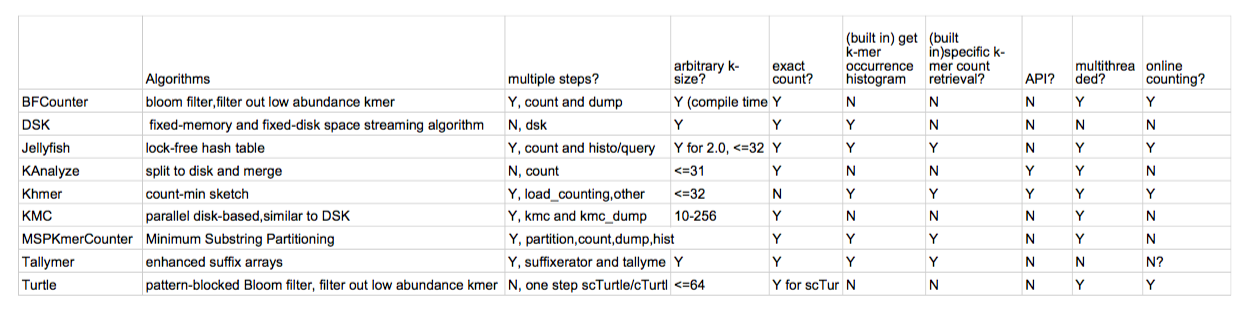
\includegraphics[width=10in]{./figures/kmer_counting.png}}

    \caption{Description of k-mer counting packages} \label{fig:kmer_counting}
    \end{sidewaysfigure}

\section{Tackling large and error-prone short-read shotgun data sets}

The ongoing improvements in DNA sequencing technologies have led to a new
problem: how do we analyze the resulting large sequence data sets quickly and
efficiently? These data sets contain millions to billions of short reads with
high error rates and substantial sampling biases \cite{pubmed19997069}.  The
vast quantities of deep sequenced data produced by these new sequencing
technologies are driving computational biology to extend and adapt previous
approaches to sequence analysis.  In particular, the widespread use of deep
shotgun sequencing on previously unsequenced genomes, transcriptomes, and
metagenomes, has resulted in the development of several new approaches to {\em
de novo} sequence assembly \cite{pubmed20211242}.

There are two major challenges in analyzing short-read sequences from shotgun
sequencing. First, deep sequencing is needed for complete sampling. This is
because shotgun sequencing samples randomly from a population of genomes;
this sampling is biased by sample content and sample preparation, requiring
even deeper sequencing. A human genome may require 100x coverage or more for
near-complete sampling, leading to shotgun data sets 300 GB or larger in
size\cite{pubmed21187386}. Since the lowest abundance genomes determines the
depth of coverage required for complete sampling, transcriptomes and
metagenomes containing rare population elements can also require similarly deep
sequencing.

The second challenge to analyzing short-read shotgun sequencing is the high
error rate.  For example, the Illumina GAII sequencer has a 1-2\% error rate,
yielding an average of one base error in every 100 bp of data
\cite{pubmed19997069}.  The total number of errors grows linearly with the
amount of data generated, so these errors usually dominate novelty in large
data sets \cite{pubmed21245053}.  Tracking this novelty and resolving errors is
computationally expensive.

These large data sets and high error rates combine to provide a third
challenge: it is now straightforward to generate data sets that cannot easily
be analyzed \cite{pubmed21867570}.  While hardware approaches to scaling
existing algorithms are emerging, sequencing capacity continues to grow faster
than computational capacity \cite{pubmed20441614}.  Therefore, new algorithmic
approaches to analysis are needed.

Many new algorithms and tools have been developed to tackle large and
error-prone short-read shotgun data sets. A new class of alignment tools, most
relying on the Burrows-Wheeler transform, has been created specifically to do
ultra-fast short-read alignment to reference sequence \cite{pubmed19430453}. 
In cases where a reference sequence does not exist and must be assembled {\em
de novo} from the sequence data, a number of new assemblers have been written,
including ABySS, Velvet, SOAPdenovo, ALLPATHS, SGA, and Cortex
\cite{pubmed19251739,pubmed18349386,pubmed20511140,pubmed21187386,
pubmed22156294,cortex}. These assemblers rely on theoretical advances to store
and assemble large amounts of data \cite{pubmed22068540,pubmed20529929}.  As
short-read sequencing has been applied to single cell genomes, transcriptomes,
and metagenomes, yet another generation of assemblers has emerged to handle
reads from abundance-skewed populations of molecules; these tools, including
Trinity, Oases, MetaVelvet, Meta-IDBA, and Velvet-SC, adopt local models of
sequence coverage to help build assemblies
\cite{pubmed21572440,pubmed22368243,metavelvet,pubmed21685107,pubmed21926975}.
In addition, several ad hoc strategies have also been applied to reduce
variation in sequence content from whole-genome amplification
\cite{pubmed19724646,pubmed22028825}. Because these tools all rely on k-mer
approaches and require exact matches to construct overlaps between sequences,
their performance is very sensitive to the number of errors present in the
underlying data. This sensitivity to errors has led to the development of a
number of error removal and correction approaches that preprocess data prior to
assembly or mapping \cite{pubmed21685062,pubmed15059830,Kelley2010}.

One approach to error correction involves finding low-abundance fixed-length
words, or k-mers, and treating them as likely errors; these errors can then be
``corrected'' by changing them to similar k-mers that are in high abundance
\cite{pubmed21114842}.  This approach requires two complete iterations across
the data set: one iteration to collect abundance spectra, and a second to
perform the trimming or correction.  For extremely large data sets, this is a
significant problem: the ``noise'' from sequencing errors drives a supra-linear
increase in the number of k-mers, so as data set size increases, the
computation and memory needed to track k-mers increases dramatically
\cite{pubmed21245053}.


K-mer spectral analysis is a powerful approach to error detection and
correction in shotgun sequencing data that uses k-mer abundances to find likely
errors in the data \cite{Pevzner2001}.  Approaches derived from spectral
analysis can be very effective: spectral error correction achieves high
accuracy, and Zhang et al. (2014) show that spectral k-mer trimming is
considerably more effective at removing errors than quality score-based
approaches \cite{quake,Zhang2014}.  However, spectral analysis is also very
compute intensive: most implementations count all the k-mers in sequencing data
sets, which can be memory- or I/O-intensive for large data sets
\cite{Zhang2014}.

Streaming and semi-streaming algorithms can offer improved algorithmic and
computational efficiency in the analysis of large data sets \cite{Charikar2004,
Cormode2005}.  Streaming algorithms typically examine the data only once, and
have small, fixed memory usage. Semi-streaming algorithms may examine the data
a few times, with memory requirements that scale sublinearly with the size of
the input data \cite{Feigenbaum2005}.  Streaming algorithms have not been
applied to k-mer spectral analysis of sequencing reads, although Melsted et al.
developed an effective streaming algorithm for calculating {\em aggregate}
statistics of k-mer distributions from sequencing data \cite{Melsted2014}, and
the Lighter error corrector uses a low-memory semi-streaming multipass approach
to do efficient error correction \cite{lighter}.


\section{Challenges in measuring diversity of metagenomics}


\subsection{Diversity measurement in Microbial Ecology}

There have been numerous mature methods and tools to measure diversity of
macroorganisms in decades of development of classic ecology. One would think
that we just need to borrow those methods to use in microbial field.
Unfortunately in reality this is not the case. The microbial communities are so
different from macroorganisms like plant or animal communities, with the number
of species many order of magnitude larger \cite{Whitman:1998aa}. This fact
raises serious sampling problems. It is extremely difficult to cover enough
fraction of the microbial community even with impressively large sample size
thanks to modern metagenomic approaches \cite{Roesch:2007aa}. In a word,
diversity measurement is a rather big challenge for microbial communities and
novel and effective methods are highly demanded \cite{Schloss:2005aa}.

\subsubsection{OTU Identification using sequence markers} To borrow the methods
of diversity measurement from classic ecology on the use of evaluating
microbial diversity, the first problem is that in microbial world, there is no
unambiguous way to define "species" \cite{Stackebrandt:2002aa}. It is
impossible to identify a microbial individual as a specific species
morphologically. In fact in metagenomics the concept of "species" has been
replaced by OTUs(Operational Taxonomic Units). An OTUs are those microbial
individuals within a certain evolutionary distance. Practically we mainly use
16S rRNA genes as the evolutionary marker genes, because 16S rRNA genes exist
universally among different microbial species and their sequences change at a
rate corresponding with the evolutionary distance. So we can describe microbial
individuals with higher than a certain percent(e.g. 97\%) 16S rRNA sequence
similarity as one OTU, or belonging to one species \cite{Schloss:2005aa}.

\subsubsection{Binning of Metagenomic Reads into OTUs}

In classic ecology dealing with samples from macroorganisms communities, before
we can use any statistical method to measure diversity, it is standard
procedure to identify the species of each individual in a sample. It is the
same for diversity measurement of microbial communities. Difference is that
here we need to place the sequences(individuals) into respective "bin" or
OTUs(species). There are two strategies to do such binning - Composition-based
or intrinsic binning approach and similarity-based or extrinsic binning
approach.

\paragraph{Composition-based approach} Lots of efforts have been put to get a
comprehensive category of reference microbial genome sequences \cite{HMScience,
Wu:2009aa}. Currently there are a large number of finished or high-quality
reference sequences of thousands of microbial species available in different
databases and this number is still increasing quickly \cite{Markowitz:2012aa,
Glass:2010aa, Wang:2007aa}. So the first intrinsic composition-based approach
is to use those reference genomes to train a taxonomic classifier and use that
classifier to classify the metagenomics reads into bins. Different statistical
approaches like Support Vector Machines \cite{Patil:2012aa}, interpolated
Markov models\cite{Brady:2011aa},naive Bayesian classifiers, and Growing Self
Organizing Maps \cite{Rosen:2011aa} were used to train the classifier. Without
using any reference sequences for the training, it is possible to use
signatures like k-mers or codon-usage to develop reference-independent
approach. The assumption is that the frequencies distribution of the signatures
are similar of the sequences from the same species. TETRA is such a
reference-independent tools using Markov models based on k-mer frequencies
\cite{Teeling:2004aa}. There is another tool using both TETRA and codon usage
statistics to classify reads \cite{Tzahor:2009aa}.


\paragraph{Similarity-based approach} The similarity-based extrinsic approach
is to find similarity between the reads sequences and reference sequences and a
tree can be built using the similarity distance information. MEGAN
\cite{Huson:2007aa} is a typical tool using this method, which reads a BLAST
file output. Other sequence alignment tools can also be used here like BowTie2
or BWA. Recently, an alternative strategy was developed, which only uses the
reference sequences with the most information rather than all the reference
sequences to do alignment. Those reference sequences include 16S rRNA genes or
some other specific marker genes. The benefit is obvious, it is more
time-efficient since there are fewer reference sequences to align to. Also, it
can provide better resolution and binning accuracy since the marker genes can
be selected carefully with the best distinguishing power. AMPHORA2
\cite{Wu:2012aa} and MetaPhlAn \cite{Segata:2012aa} are two typical tools using
this strategy.



\subsubsection{Statistics for Diversity Estimation} After the binning of
sequences into OTU, we need statistical analysis to help us estimate the diversity. Many
statistical methods have been developed and widely used in classical ecology of
macroorganisms. However the first difference between diversity measurement of
macroorganisms and microbial community is that generally the microbial
community diversity is much larger than observed sample diversity, thanks to
the high diversity characteristics of microbial community and the limit of
metagenomics sampling and sequencing. The first approach which is also
considered as classic is rarefaction. Rarefaction curve can be used to compare
observed richness among different samples that have been sampled unequally,
which is basically plotting of the number of observed species as a function of
the sampled individuals. It is worth noting that rarefaction curve shows the
observed diversity, not the total diversity. We should not disregard those
unseen microbial species, which is pretty common for microbial community
sampling.

To estimate the total diversity from observed diversity, different estimators
are required.

The first one is extrapolation from accumulation curve. The asymptote of this
curve is the total diversity, which means the number of species will not
increase any more with sampling more individuals. To get the value of that
asymptote point, from observed accumulation curve, a function needs to be
assumed to fit the curve. Several proposals have been made to use this
extrapolation method \cite{colwell2004interpolating, gotelli2001quantifying}.
The problem is that if the sampling effort only covers a small fraction of the
total sample, which means the accumulation curve just starts, it is difficult
to find an optimal function to fit the curve. Different functions can fit the
curve equally well but will deduct dramatically different asymptote value. So
this curve extrapolation method should be used cautiously.

Another one is parametric estimator, which assumes that the relative abundance
follows a particular distribution. Then the number of unobserved species in the
community can be estimated by fitting observed sample data to such abundance
distribution then the total number of species in the community can be
estimated. Lognormal abundance distribution is mostly used in different project
since most communities of macroorganisms has a lognormal abundance distribution
and it is believed that it is also typical for some microbial communities
\cite{Curtis:2002aa, Schloss:2006aa, Quince:2008aa}. It is understandable that
there is always controversy as to which models fit the communities best since
in an ideal world the abundance distribution should be inferred from the
data,not be assumed unverifiably. The problem is that we can only infer the
abundance distribution accurately when the sample size is large enough. There
have been some attempts on this direction recently \cite{Gans:2005aa} and more
robust methods are still needed.

If the species abundance distribution can not be inferred, we can still use
nonparametric estimators to estimate the total diversity without assuming that
abundance distribution arbitrarily. These estimators are related to
MRR(mark-release-recapture) statistics, which compare the number of species
observed more than once and the number of species observed only once. If
current sampling only covers a small fraction of a diverse community, the
probability that a species is observed more than once will be low and most
species will be observed only once. If current sampling is enough to cover most
species in the community, the opposite will be the case. A series of estimators
invented by Chao are the representative estimators in this category, including
Chao1 \cite{chao1984nonparametric}, Chao2 \cite{Chao:1987aa}, ACE
\cite{chao1993stopping} and ICE \cite{lee1994estimating}. For example, Chao1
formular is:\\ $${S}_{Chao1}={S}_{obs}+\frac{{{n}_{1}}^{2}}{2{n}_{2}}$$ where
${S}_{obs}$ is the number of species observed, ${n}_{1}$ the number of species
observed once(singletons, with only one individule), and ${n}_{2}$ the number
of species observed twice(doubletons, with exactly two individuals) in the
sample. The ACE uses data from all species rather than just singletons and
doubletons. Its formular is:\\
$${S}_{ACE}={S}_{abund}+\frac{{S}_{rare}}{{C}_{ACE}}+\frac{{F}_{1}}{{C}_{ACE}}{
{\gamma }_{ACE}}^{2}$$ where ${S}_{rare}$ is the number of rare species (with
few than 10 individuals observed) and ${S}_{abund}$ is the number of abundant
species (with more than 10 individuals).

In past years there are several software packages that have been developed for
biodiversity analysis. Out of them, EstimateS \cite{colwellestimates} is a
software that can be used for general purpose diversity analysis, which
implement a rich set of diversity analysis algorithms. However it is not
designed specifically for microbial diversity analysis. So microbial diversity
data should be preprocessed to general population data to be fed into
EstimateS. Two other softwares - MOTHUR \cite{Schloss:2009aa} and QIIME
\cite{Caporaso:2010aa} are designed for microbial diversity. So they are more
popular in microbial diversity analysis. CatchAll \cite{Bunge:2011aa} is a
relatively newer package, which can estimate the diversity using both
nonparametric and parametric estimators including many variants and return the
results using different estimators and the respective credibility of the
results.


